\documentclass[a4paper,12pt]{article}

\usepackage{graphicx} % Required for inserting images
\usepackage{amsmath,amssymb,amsfonts}
\usepackage{subcaption}
% -----------------------
% Package Imports
% -----------------------

% Set page margins
\usepackage[a4paper, top=1in, bottom=0.8in, left=1.1in, right=0.8in]{geometry}

% Use Times New Roman font
\usepackage{times}

% Add page numbering
\pagestyle{plain}
\usepackage{multirow}
% Enable graphics inclusion
\usepackage{graphicx}
\usepackage{float}
% Enable code listings
\usepackage{listings}
\usepackage{xcolor} % For customizing code colors

% Define MATLAB style for listings
\lstdefinestyle{vscode-light}{
	language=Matlab,
	basicstyle=\ttfamily\footnotesize,
	keywordstyle=\color{black},
	commentstyle=\color{gray},
	stringstyle=\color{red},
	numberstyle=\tiny\color{black},
	numbersep=5pt,
	frame=single,
	backgroundcolor=\color{white!10},
	breaklines=true,
	captionpos=b,
	tabsize=4,
	showstringspaces=false,
	numbers=left,  % Enable line numbering on the left
	stepnumber=1,  % Line numbers increment by 1
	numberfirstline=true, % Number the first line
}
\setlength{\parindent}{0pt}
\usepackage{titlesec} % To customize section font size
\titleformat{\section}
{\normalfont\fontsize{14}{16}\bfseries}{\thesection}{1em}{}

\titleformat{\subsection}
{\normalfont\fontsize{14}{16}\bfseries}{\thesubsection}{1em}{}


\begin{document}
	\section{Experiment No. 3}
	
	\section{Experiment Title }
Observation \& Verification of Frequency Modulation and Demodulation
	\section{Objective}
	

	
The objectives of this lab are as follows:
\begin{itemize}
	\item To understand how the frequency of the carrier wave varies according to the message
	signal.
	\item To demodulate the FM signal and recover the original message signal.
\end{itemize}

	\section{Theory}
	
	\subsection{Frequency Modulation (FM)}
	
	Frequency Modulation (FM) is a technique of modulating a carrier signal in which the frequency of the carrier wave is varied in accordance with the instantaneous amplitude of the modulating (message) signal, while its amplitude remains constant. The general expression for an FM signal is:
	
	\begin{equation}
		s(t) = A_c \cos\left(2\pi f_c t + 2\pi k_f \int_0^t m(\tau) d\tau \right)
		\label{eq:fm_signal}
	\end{equation}
	
	Where:
	\begin{itemize}
		\item $A_c$ is the amplitude of the carrier signal
		\item $f_c$ is the carrier frequency
		\item $k_f$ is the frequency sensitivity (Hz/V)
		\item $m(t)$ is the modulating signal
	\end{itemize}
	
	The instantaneous frequency of the FM signal is given by:
	
	\begin{equation}
		f_i(t) = f_c + k_f m(t)
	\end{equation}
	
	Thus, the frequency of the carrier varies with the amplitude of the input signal $m(t)$.
	
	\subsection{Modulation Index in FM}
	
	The modulation index ($\beta$) in FM is defined as the ratio of frequency deviation ($\Delta f$) to the modulating frequency ($f_m$):
	
	\begin{equation}
		\beta = \frac{\Delta f}{f_m}
	\end{equation}
	
	\subsection{Demodulation of FM Signal}
	
	FM demodulation is the process of recovering the original modulating signal from the frequency-modulated carrier. This can be achieved using different techniques such as:
	\begin{itemize}
		\item Frequency discriminator
		\item Phase-locked loop (PLL)
	\end{itemize}
	
	One common approach is using a frequency discriminator which converts frequency variations into amplitude variations, followed by an envelope detector to recover the original signal.
	
	Alternatively, a Phase-Locked Loop (PLL) based demodulator uses a voltage-controlled oscillator (VCO) that locks onto the frequency of the input FM signal and produces an output voltage proportional to the frequency deviation, hence reproducing the modulating signal.
	
	\subsection{Bandwidth of FM Signal}
	
	According to Carson’s Rule, the bandwidth ($B$) required for an FM signal is given by:
	
	\begin{equation}
		B = 2(\Delta f + f_m) = 2f_m(\beta + 1)
	\end{equation}
	
	This shows that FM requires a wider bandwidth than AM, especially when the modulation index is large.
	
	
	\subsection{Required Apparatus}
	\begin{enumerate}
		
		\item DCTK-1000 \& ACTK-1000 kit.
		\item	Digital Oscilloscope (TBS-1000c).
		\item Connecting wires \& Probes.
	\end{enumerate}
	
	\newpage
	\subsubsection{MATLAB Code:}
	\begin{lstlisting}[style=vscode-light, caption={Frequency Modulation.} ]
	clear all;
	close all;
	
	% Parameters
	t = 0:0.0001:0.1;      % Time vector
	fm = 50;               % Message signal frequency (Hz)
	fc = 500;              % Carrier signal frequency (Hz)
	Am = 1;                % Message amplitude
	Ac = 1;                % Carrier amplitude
	kf = 100;              % Frequency sensitivity (Hz/V)
	
	% Message Signal
	m_t = Am * cos(2 * pi * fm * t);      
	
	% Carrier Signal
	c_t = Ac * cos(2 * pi * fc * t);      
	
	% Frequency Modulated Signal
	dt = t(2) - t(1); 
	int_m_t = cumsum(m_t) * dt; % Integration of message signal
	s_fm = Ac * cos(2 * pi * fc * t + 2 * pi * kf * int_m_t); % FM signal
	
	% Plot Message Signal (Green)
	figure('Position', [100, 100, 600, 400]);
	plot(t, m_t, 'g', 'LineWidth', 1.5);
	title('Message Signal');
	xlabel('Time (s)');
	ylabel('Amplitude');
	grid on;
	set(gcf, 'Color', 'w');
	
	% Plot Carrier Signal (Red)
	figure('Position', [750, 100, 600, 400]);
	plot(t, c_t, 'r', 'LineWidth', 1.5);
	title('Carrier Signal');
	xlabel('Time (s)');
	ylabel('Amplitude');
	grid on;
	set(gcf, 'Color', 'w');
	
	% Plot FM Signal (Black)
	figure('Position', [400, 550, 600, 400]);
	plot(t, s_fm, 'k', 'LineWidth', 1.5);
	title('Frequency Modulated (FM) Signal');
	xlabel('Time (s)');
	ylabel('Amplitude');
	grid on;
	set(gcf, 'Color', 'w');
	
	
	
		
		
	\end{lstlisting}
	\section{Plot Diagram}
	\begin{figure}[H]
		\centering
		\begin{subfigure}[t]{0.49\textwidth}
			\centering
			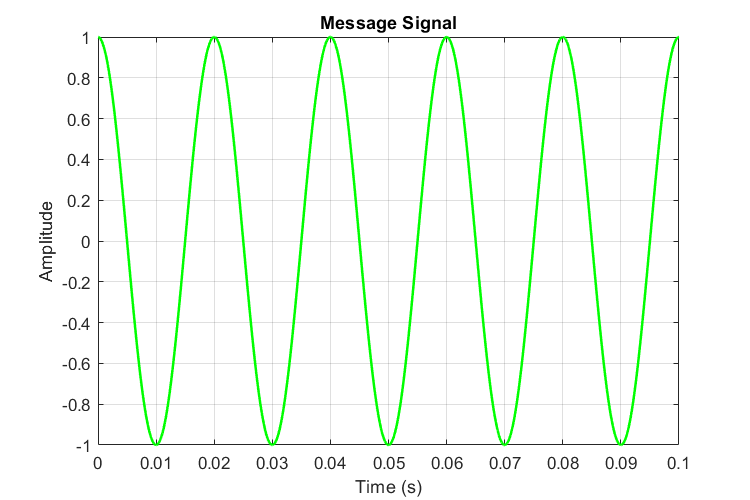
\includegraphics[width=1\linewidth]{Images/1}
			\caption{Message Signal}
			\vspace{0.1cm}
		\end{subfigure}
		\hfil
		\begin{subfigure}[t]{0.49\textwidth}
			\centering
			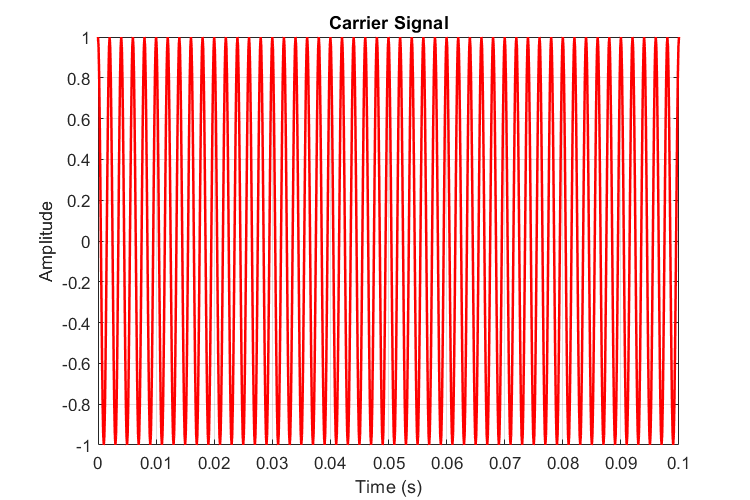
\includegraphics[width=1\linewidth]{Images/2}
			\caption{ Carrier Signal}
		\end{subfigure}
		
		\begin{subfigure}[t]{0.49\textwidth}
			\centering
			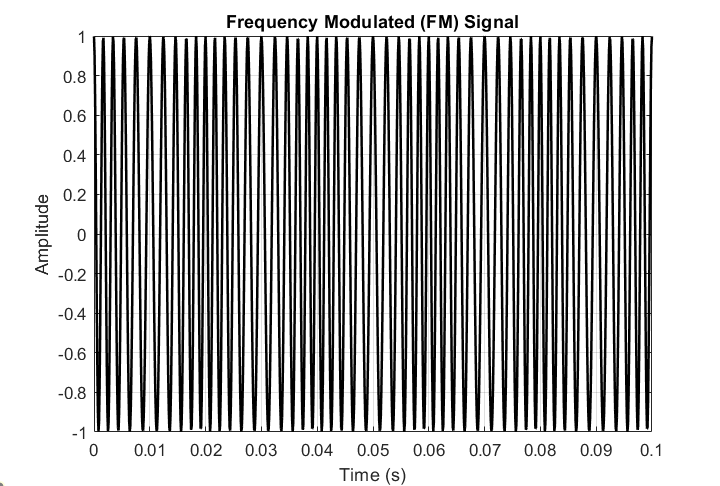
\includegraphics[width=1\linewidth]{Images/3.1}
			\caption{ Modulated signal }
		\end{subfigure}
	
	\end{figure}
	
	
	\section{Experimental Setup}
	\begin{figure}[H]
		\centering
		
		
		\begin{subfigure}[t]{0.81\textwidth}
			\centering
			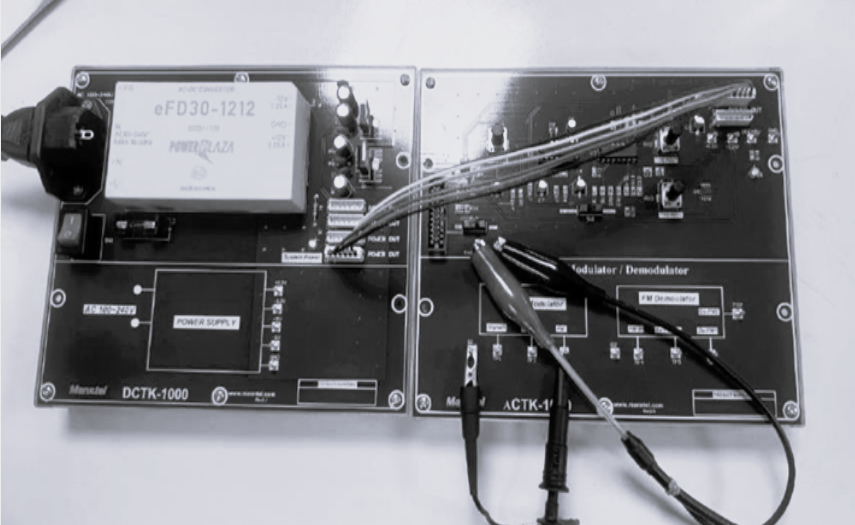
\includegraphics[width=0.85\linewidth]{Images/4.1}
			\caption{ Actual setup}
		\end{subfigure}
			\begin{subfigure}[t]{0.81\textwidth}
			\centering
			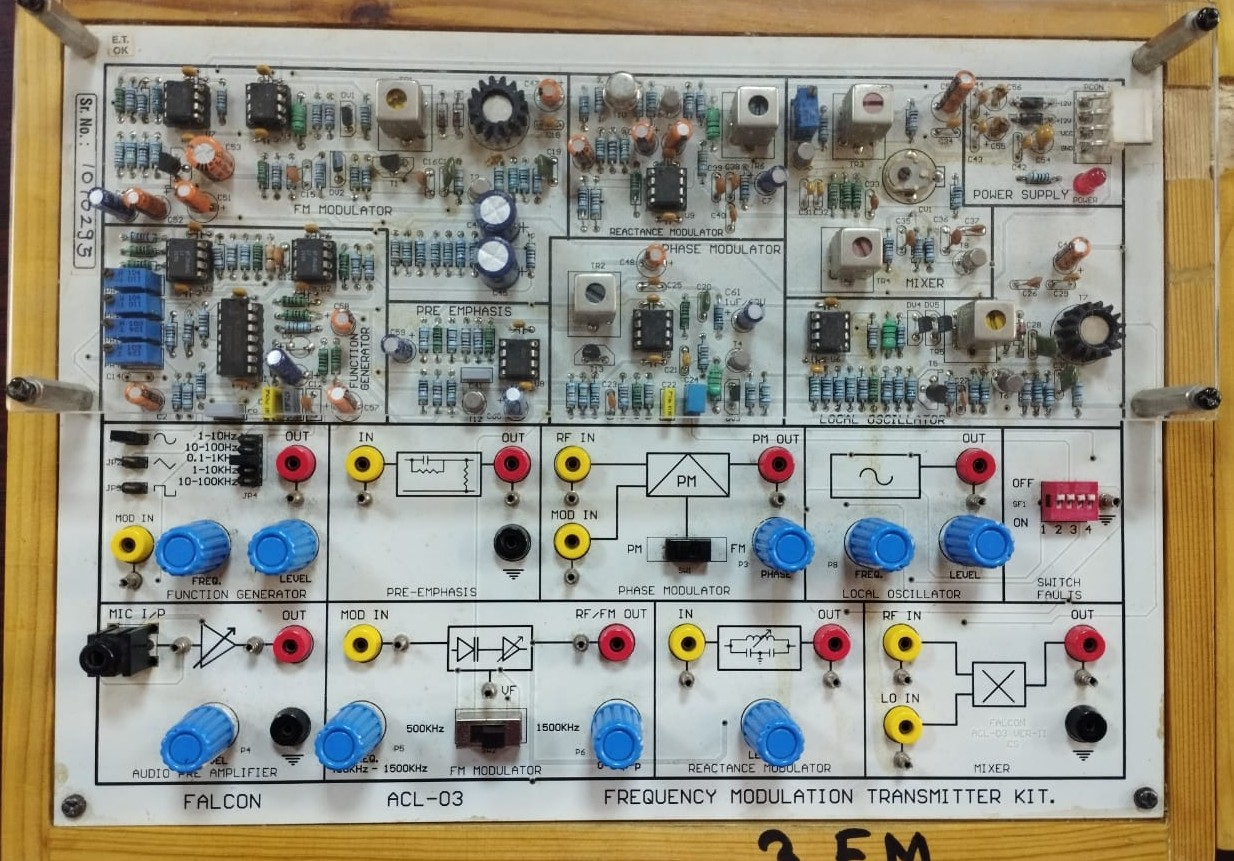
\includegraphics[width=0.85\linewidth]{Images/13}
			\caption{ Actual setup}
		\end{subfigure}
		\begin{subfigure}[t]{0.81\textwidth}
			\centering
			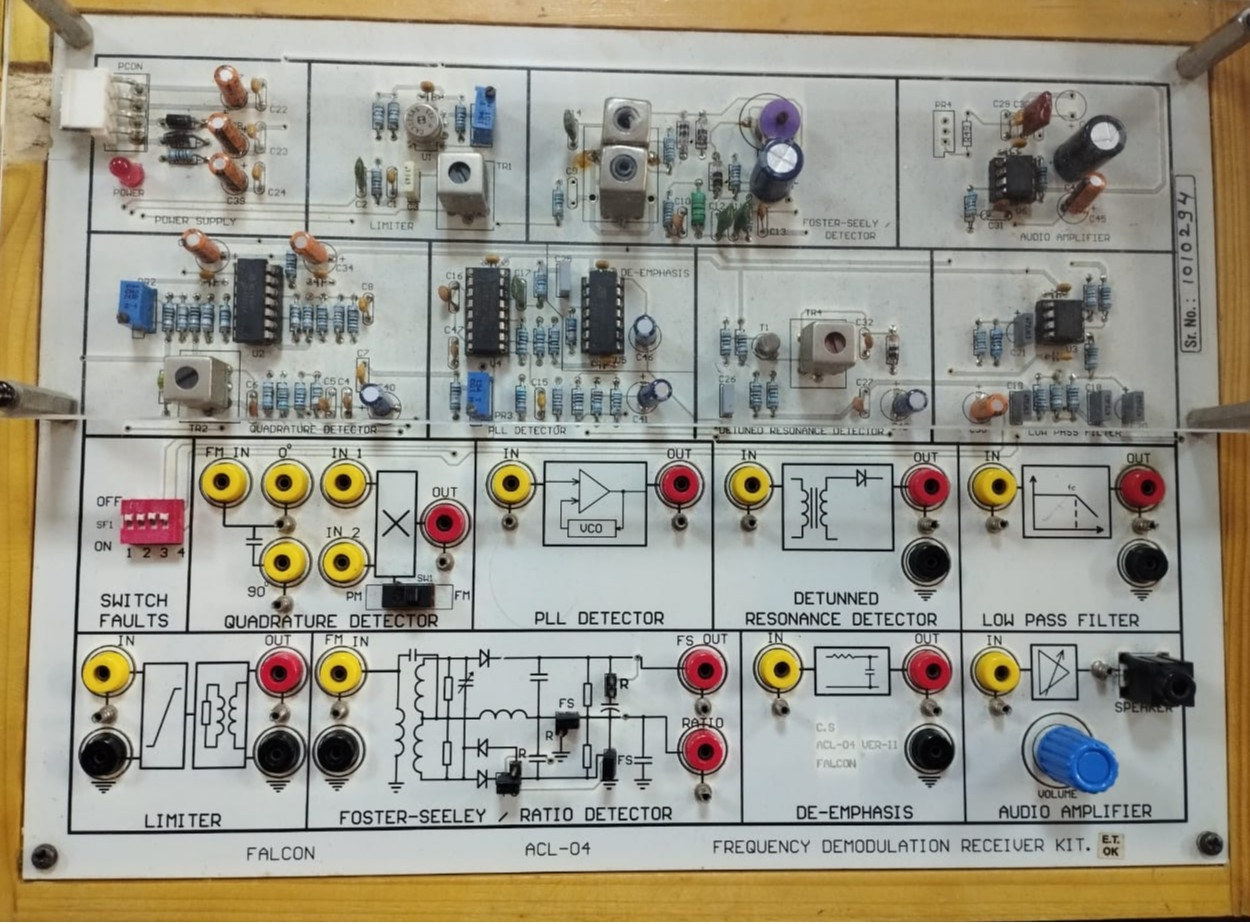
\includegraphics[width=0.85\linewidth]{Images/14}
			\caption{ Actual setup}
		\end{subfigure}
	\end{figure}
	
	
	

	
	
	
	\section{Experimental Wavehape}
	\begin{figure}[H]
	\centering
	\begin{subfigure}[t]{0.7\textwidth}
		\centering
		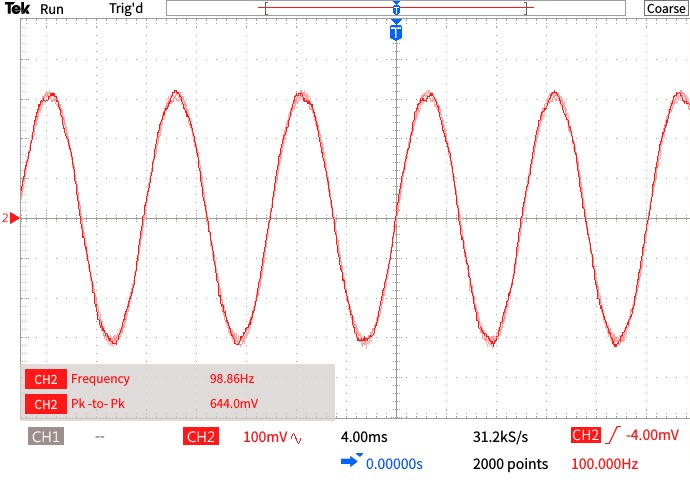
\includegraphics[width=1\linewidth]{Images/5.1}
		\caption{Message Signal}
		\vspace{0.1cm}
	\end{subfigure}

	\begin{subfigure}[t]{0.7\textwidth}
		\centering
		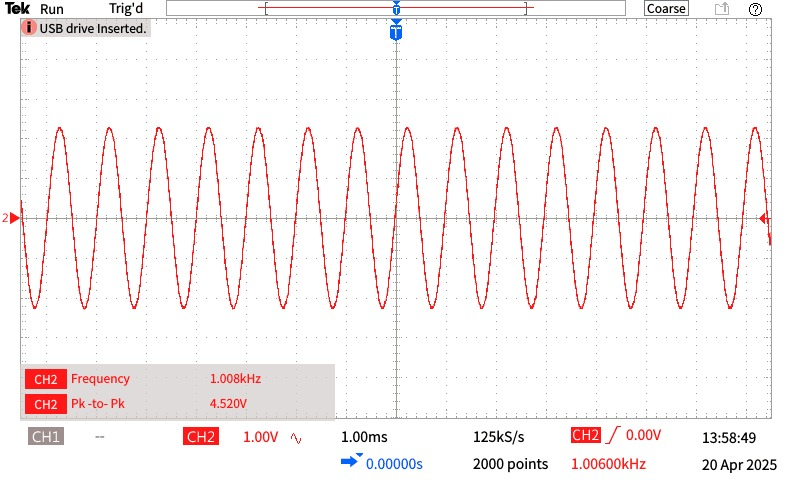
\includegraphics[width=1\linewidth]{Images/6}
		\caption{ Carrier Signal}
	\end{subfigure}
	
	\begin{subfigure}[t]{0.7\textwidth}
		\centering
		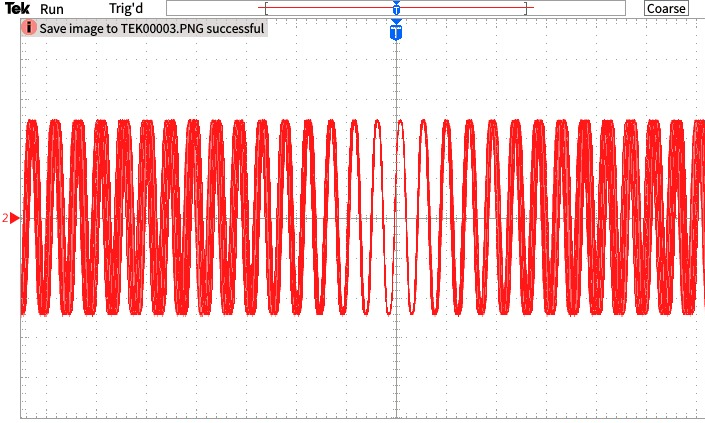
\includegraphics[width=1\linewidth]{Images/7}
		\caption{ Modulated signal }
	\end{subfigure}

	
\end{figure}

\newpage
	\begin{figure}[H]
	\centering
	
	
	\begin{subfigure}[t]{0.49\textwidth}
		\centering
		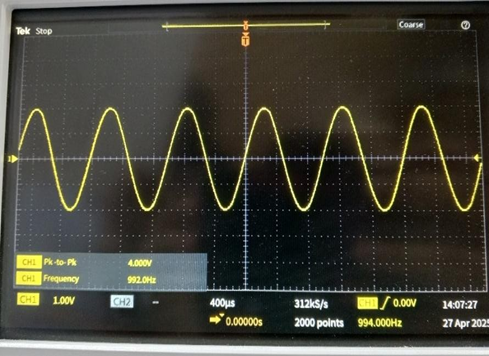
\includegraphics[width=1\linewidth]{Images/9}
		\caption{Message signal Frequency 992 Hz   ,                                    Peak to Peak Voltage 4V 
		}
	\end{subfigure}
	\hfil
	\begin{subfigure}[t]{0.49\textwidth}
		\centering
		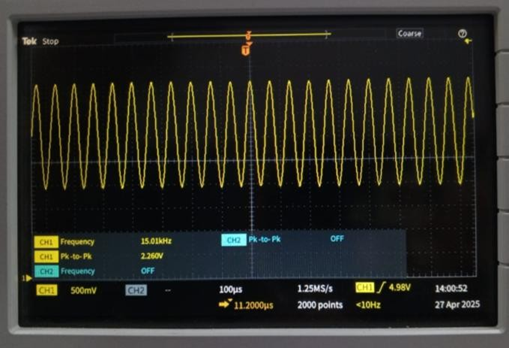
\includegraphics[width=1\linewidth]{Images/10}
		\caption{ Carrier signal Frequency 15010 Hz,               
		                                         Peak to Peak Voltage 2.26 V
		}
	\end{subfigure}
	\begin{subfigure}[t]{0.49\textwidth}
		\centering
		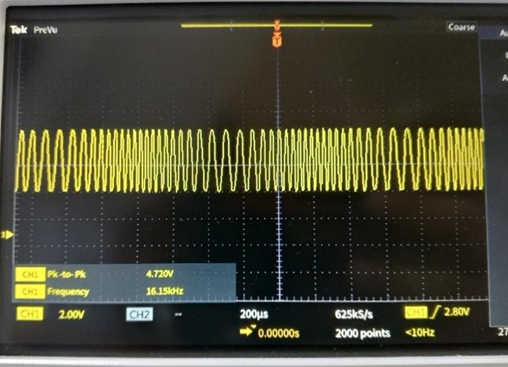
\includegraphics[width=1\linewidth]{Images/11}
		\caption{Modulated Signal Frequency 16.15 kHz,                        
			Peak to Peak Voltage 4.72 V 
		}
	\end{subfigure}
	\hfil
	\begin{subfigure}[t]{0.49\textwidth}
		\centering
		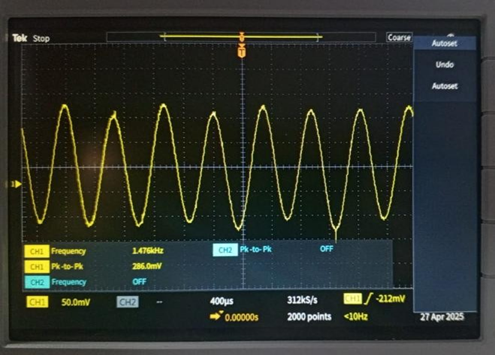
\includegraphics[width=1\linewidth]{Images/12}
		\caption{ Demodulated Signal Frequency 1.476 kHz,               
		                                  Peak to Peak Voltage 286 mV
		}
	\end{subfigure}
\end{figure}


\begin{figure}
	\centering
\begin{subfigure}[t]{0.7\textwidth}
	\centering
	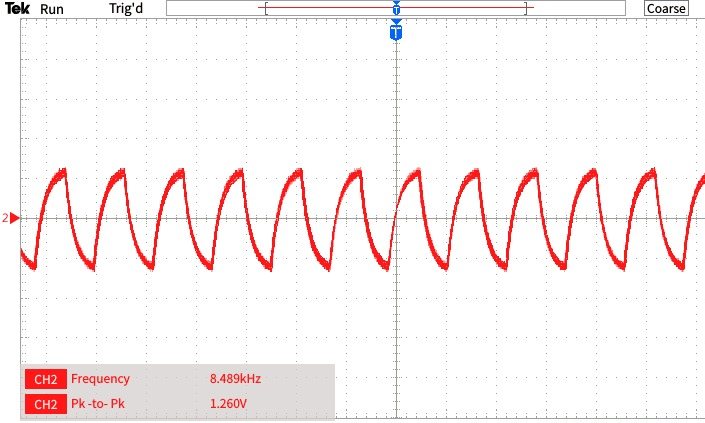
\includegraphics[width=1\linewidth]{Images/8}
	\caption{ Demodulated signal }
\end{subfigure}
\end{figure}
	\newpage

\section{Discussion}
In the experiment, frequency modulation and demodulation were observed using a frequency‐modulation transmitter kit and a frequency‐demodulation receiver kit. The transmitter circuit was assembled as per the provided manual, where both the message and carrier signals were generated using signal generators. These signals were used to produce a frequency modulated waveform by varying the instantaneous frequency of the carrier in accordance with the amplitude of the message signal. The modulated signal was then transmitted to the demodulation kit. The receiver employed a frequency discriminator circuit, which successfully recovered the original message signal from the modulated waveform, demonstrating the working principle of frequency modulation and demodulation.

	
	\newpage
	
	
\end{document}